\section{Results and Discussion}

\begin{figure}[H]
	\centering
	\begin{subfigure}{\textwidth}
		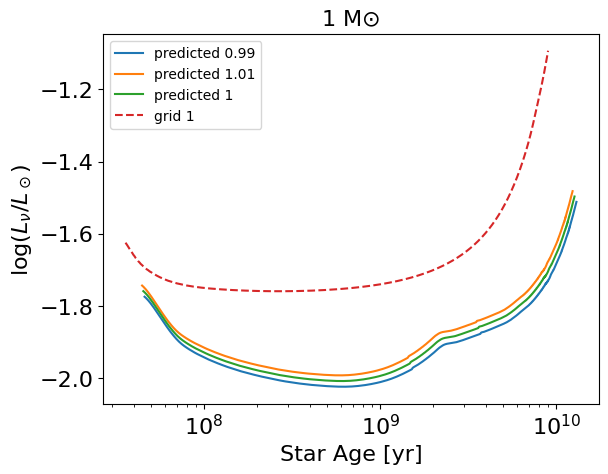
\includegraphics[width=\textwidth,height=0.5\textheight]{assets/output1singlemodel.png}
		\caption{Sun $1M\odot$ Single Testing Data.}
		\label{fig:SunTesta}	
	\end{subfigure}
	\begin{subfigure}{\textwidth}
		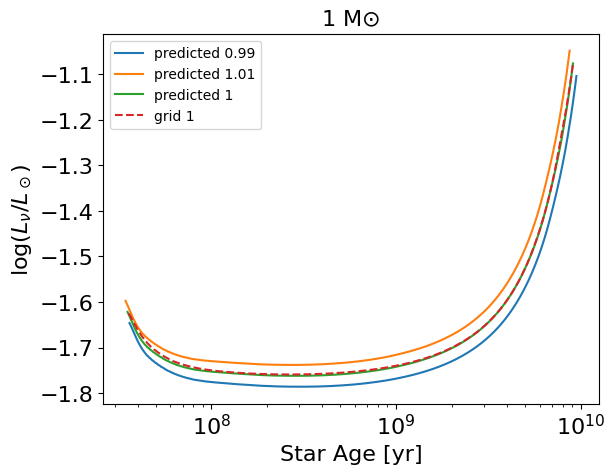
\includegraphics[width=\textwidth,height=0.5\textheight]{assets/output1.png}
		\caption{Sun $1M\odot$ Multi Model($0.5-1.1M_\odot$) Testing Data.}
		\label{fig:SunTestb}	
	\end{subfigure}
	\label{fig:SunTest}
\end{figure}

\begin{figure}[H]
	\centering
	\begin{subfigure}{\textwidth}
		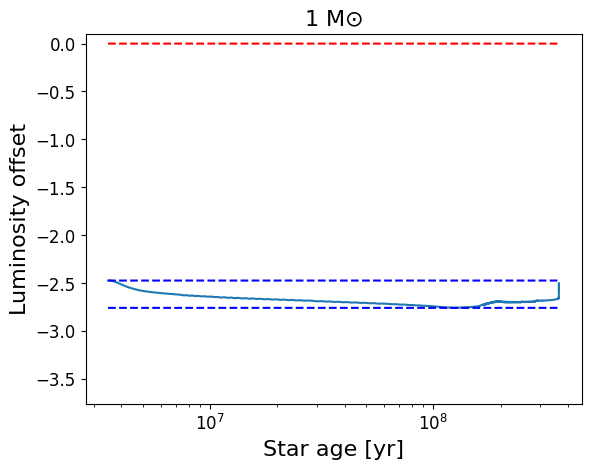
\includegraphics[width=\textwidth,height=0.5\textheight]{assets/error1modelsingle.png}
		\caption{Luminosity Offset for $1M\odot$.}
	\end{subfigure}
	\begin{subfigure}{\textwidth}
		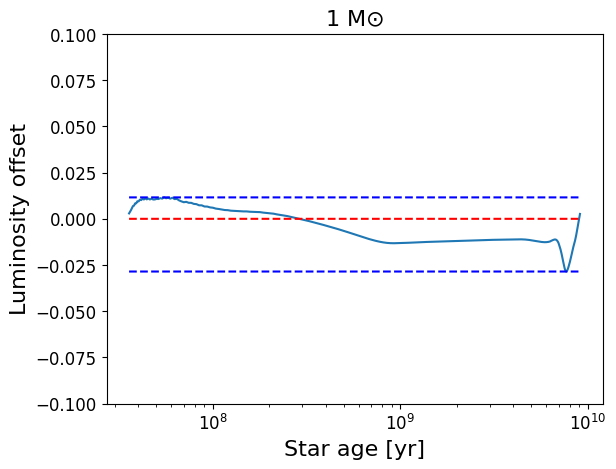
\includegraphics[width=\textwidth,height=0.5\textheight]{assets/error 1.png}
		\caption{Single Multimodel Error.}	
\end{subfigure}
	\label{fig:lumoff}
\end{figure}

\begin{figure}[H]
	\centering
	\begin{subfigure}{\textwidth}
		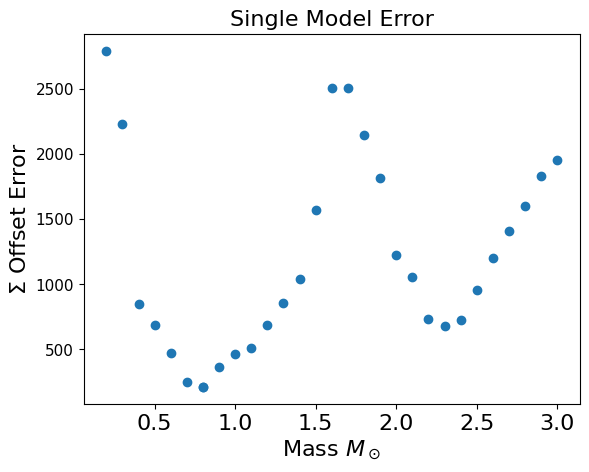
\includegraphics[width=\textwidth,height=0.5\textheight]{assets/singlemodeerror.png}
		\caption{Single Model Error.}
	\end{subfigure}
	\begin{subfigure}{\textwidth}
		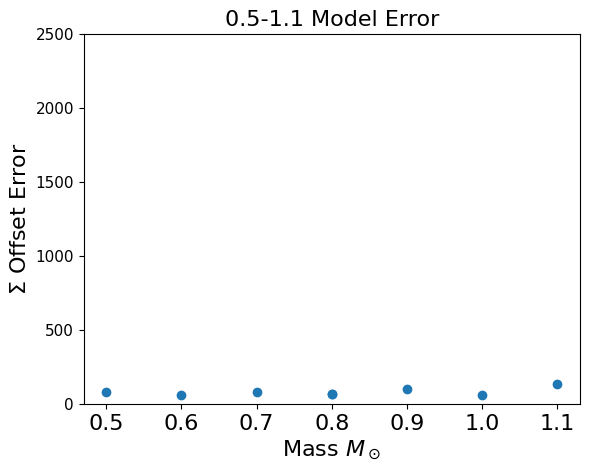
\includegraphics[width=\textwidth,height=0.5\textheight]{assets/0.5-1.1Error.png}
		\caption{$0.5-1.1M\odot$ Model Error.}
	\end{subfigure}
	\label{fig:sumerror}
\end{figure}

\begin{table}[H]
    \centering
	\caption{Stars with their mass and distance.}
	\label{tab:stars and mass}
	\begin{tabular}{ccc}
		\toprule
		Star & Mass [$M\odot$]  & Distance [$pc$] \\
		\midrule
		$\tau$ ceti & $0.78$ & $3.65$\\
		Sun & $1$ & $4.85\times 10^{-6}$\\
		 & $1$ & $4.85\times 10^{-6}$\\
		\bottomrule
	\end{tabular}
\end{table}

\begin{figure}[H]
	\centering
	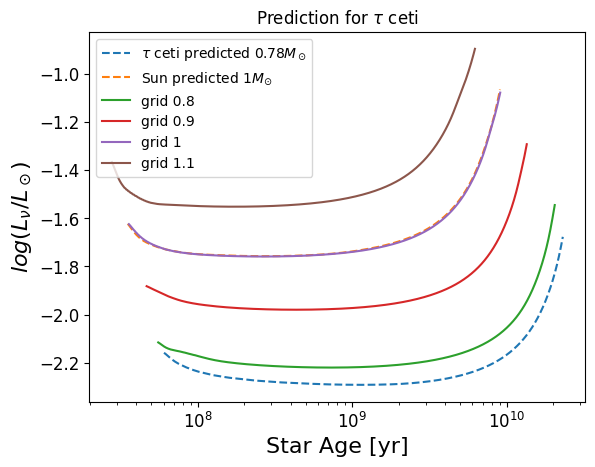
\includegraphics[width=\textwidth,height=0.5\textheight]{assets/predtauceti.png}
	\caption{Prediction for $\tau$ ceti $0.78 M\odot$.}
	\label{fig:tau}
\end{figure}

\begin{figure}[H]
	\centering
	\begin{subfigure}{\textwidth}
		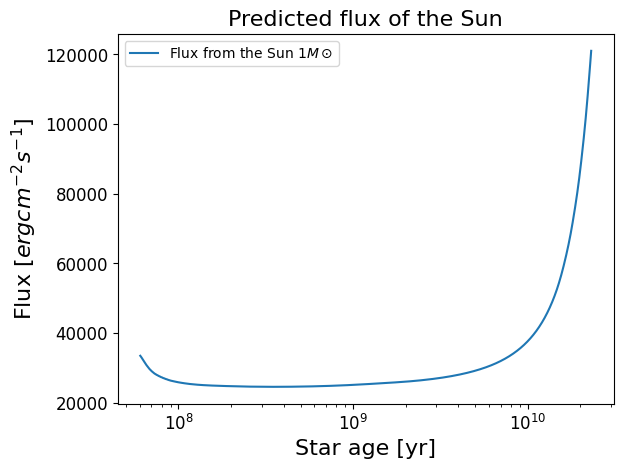
\includegraphics[width=\textwidth,height=0.5\textheight]{assets/fluxsun.png}
		\caption{Prediction for Flux of Sun $1 M\odot$.}
	\end{subfigure}
	\begin{subfigure}{\textwidth}
		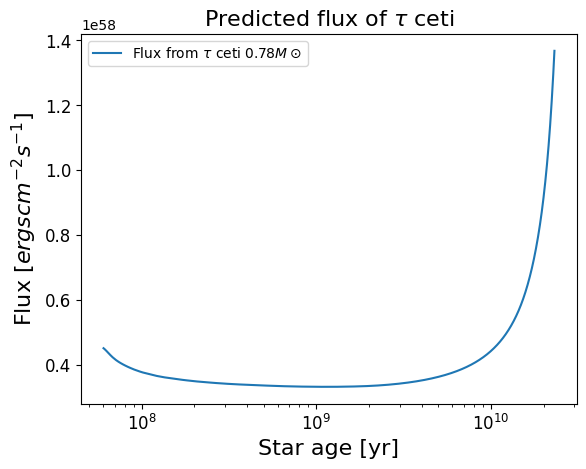
\includegraphics[width=\textwidth,height=0.5\textheight]{assets/fluxtau.png}
		\caption{Prediction for flux of $\tau$ ceti $0.78 M\odot$.}
	\end{subfigure}
	\label{fig:predicted flux}
\end{figure}
